% !TEX program = xelatex

\documentclass[10pt,a4paper]{article}
\usepackage[top = 1.5cm, bottom = 1.5cm, left = 1.5cm, right = 1.5cm]{geometry}
\usepackage{wrapfig}
\usepackage{float}

\usepackage{titling}
\usepackage[czech]{babel}
\usepackage{graphicx}
\usepackage{lmodern}
\usepackage{hyperref}
\usepackage{setspace}
\usepackage{csvsimple}

\usepackage{amsmath}
\usepackage{amssymb}
\usepackage{gensymb}
\usepackage{mathtools}
\usepackage{units}
\usepackage{bm}
\delimitershortfall=-1pt



% redefine \sqrt
\usepackage{letltxmacro}
\makeatletter
\let\oldr@@t\r@@t
\def\r@@t#1#2{%
\setbox0=\hbox{$\oldr@@t#1{#2\,}$}\dimen0=\ht0
\advance\dimen0-0.2\ht0
\setbox2=\hbox{\vrule height\ht0 depth -\dimen0}%
{\box0\lower0.4pt\box2}}
\LetLtxMacro{\oldsqrt}{\sqrt}
\renewcommand*{\sqrt}[2][\ ]{\oldsqrt[#1]{#2\,}\,}
\makeatother



\DeclarePairedDelimiter\ceil{\lceil}{\rceil}
\DeclarePairedDelimiter\floor{\lfloor}{\rfloor}

\def\ph{\phantom}
\def\vph{\vphantom}
\def\hph{\hphantom}
\def\rzw{\mathrlap}
\def\lzw{\mathllap}
\def\czw{\mathclap}

\def\?{\mathit{?}}

\def\+{+\!\!}
\def\-{-\!\!}

\newcommand{\comm}[2]{\left[ #1, #2 \right]}
\newcommand{\const}[1]{\text{#1}}
\newcommand{\norm}[1]{\left\lVert#1\right\rVert}

\newcommand{\mat}[1]{
    \begin{pmatrix}
        #1
    \end{pmatrix}
}

\newcommand{\mata}[2]{
    \left(
    \begin{array}{@{}#1@{}}
        #2
    \end{array}
    \right)
}

\newcommand{\smat}[2][1]{
    \scalebox{#1}{$\mat{#2}$}
}

\newcommand{\tg}{\operatorname{tg}}
\newcommand{\cotg}{\operatorname{cotg}}
\newcommand{\Res}{\operatorname{Res}}
\renewcommand{\Re}{\operatorname{Re}}

\renewcommand{\d}[1]{\;\const{d}#1}
\newcommand{\dd}[2]{\frac{\const{d} #1}{\const{d} #2} \;}
\newcommand{\pd}[2]{\frac{\partial  #1}{\partial  #2} \;}

\newcommand{\bra}[1]{\left< #1 \right|}
\newcommand{\ket}[1]{\left| #1 \right>}
\newcommand{\braket}[2]{\left< #1 \middle| #2 \right>}

\newcommand{\bhat}[1]{\hat{\bm{#1}}}

\newcommand{\e}[1]{\const{e}^{#1}}
\renewcommand{\i}{\const{i}}

\newcommand{\concurrent}{{\upharpoonleft\!\upharpoonright}}
\newcommand{\countercurrent}{{\upharpoonleft\!\downharpoonright}}

\newcommand{\textmath}[2]{\texorpdfstring{$#2$}{#1}}

\begin{document}

\title{Matematika pro Fyziky 2: DÚ 2}
\author{Michal Grňo}
\date{\today}

\maketitle

\section{Příklad 6}
\subsection{Zadání}
\begin{equation*}
    I = \int_{-\infty}^{+\infty} \frac{1}{(x^2+a^2)(x^2+b^2)^2},
    \hspace{2em}
    a, b \in \mathbb{R}
\end{equation*}
\subsection{Řešení}
Integrovanou funkci si rozšíříme na $\mathbb{C}$. Vidíme, že je holomorfní až na konečný počet singularit. Rozkladem jmenovatele nalezneme, kde leží její singularity:
\begin{equation*}
    (x^2+a^2)(x^2+b^2)^2 = (x+\i a)(x-\i a)(x+\i b)^2(x-\i b)^2
\end{equation*}
Máme tedy jednonásobné kořeny $\pm \i a$ a dvojnásobné kořeny $\pm \i b$.

Hodnotu integrálu $I$ vypočteme pomocí křivkového integrálu v komplexní rovině. Budeme integrovat po křivce $\varphi = \varphi_1 \oplus \varphi_2$:
\begin{figure}[H]
    \centering
    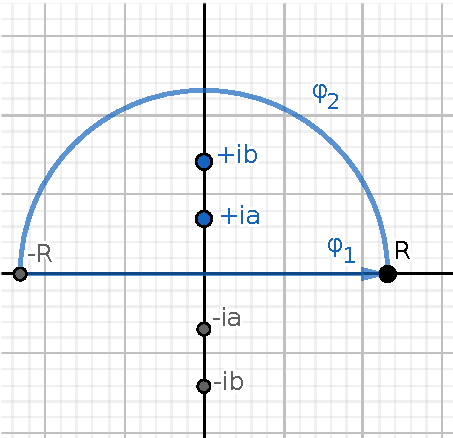
\includegraphics[width=0.4\textwidth]{du2u1param.pdf}
    \label{obr:du2u1param}
\end{figure}
\begin{gather*}
    f(z) = \frac{1}{(z^2+a^2)(z^2+b^2)^2},
    \hspace{2em}
    \int_\varphi f \d{z} = \int_{\varphi_1} f \d{z} + \int_{\varphi_2} f \d{z}
    \\[5pt]
    \varphi_1 = t \mapsto Rt, t \in [-1, 1],
    \hspace{2em}
    \varphi_2 = t \mapsto R\e{it}, t \in [0, \pi]
\end{gather*}
Pro dostatečně velkou počáteční volbu $R$ budou obě singularity uvnitř integrované oblasti. Nyní vypočteme $\int_\varphi f \d{z}$ pomocí reziduové věty, nejprve za předpokladu, že $a\neq b$:
\begin{align*}
    \int_\varphi f \d{z}
    &= 2\pi\i \left( \Res_{\i a} f + \Res_{\i b} f \right) \\
    &= 2\pi\i \left(
        \frac{1}{2a\i} \frac{1}{(b^2 - a^2)} +
        \lim_{z \to \i b} \,\dd{}{z}\! \frac{(z- \i b)^2}{(z^2+a^2)(z^2+b^2)^2}
    \right) \\[5pt]
    &= 2\pi\i \left(
        -\frac{\i}{2a(b^2 - a^2)} +
        \frac{\i (3b^2 - a^2)}{4b^3 (a^2 - b^2)}
    \right)
    \\[5pt]
    &= \frac{\pi}{(b^2 - a^2)} \left( \frac{1}{a} + \frac{3b^2 - a^2}{2b^3} \right)
    \;\;\; = \;\;\; \pi \frac{2b^3 + 3ab^2 - a^3}{2ab^3 (b^2 - a^2)}.
\end{align*}

Nyní vyšetříme případ $a=b$:
\begin{align*}
    \int_\varphi f \d{z}
    &= 2\pi\i \Res_{\i a} f
    = 2\pi\i \; \lim_{z \to \i a} \; \frac{1}{2} \; \dd{^2}{z^2} \frac{(z-\i a)^3}{(z^2 + a^2)^3}
    \\[5pt]
    &= \pi \i \lim_{z \to \i a} \; -3 \; \dd{}{z} \frac{1}{(z + \i a)^4}
    = 3\pi\i \lim_{z \to \i a} \frac{4}{(z+\i a)^5}
    = \frac{3\pi}{8a^5}.
\end{align*}

Nyní učiníme limitní přechod $R \to \infty$:
\begin{align*}
    & \int_\varphi f \d{z} = \const{konst.} \\[5pt]
    & \int_{\varphi_1} f \d{z} \to \int_{-\infty}^{+\infty} f \d{z} \\[5pt]
    & \int_{\varphi_2} f \d{z} \to 0
\end{align*}
Že jde integrál přes $\varphi_2$ skutečně do nuly nám říká Jordanovo lemma, protože $R M_R \sim R^{-5}$. Dostáváme tedy:
\begin{align*}
    \int_\varphi f \d{z} &= \int_{\varphi_1} f \d{z} + \int_{\varphi_2} f \d{z}
    \\[5pt]
    \int_\varphi f \d{z} &= I + 0
    \\[5pt]
    I &= \begin{cases}
        a = b: \; \dfrac{3\pi}{8a^5}
        \\ \\
        a\neq b: \; \pi \dfrac{2b^3 + 3ab^2 - a^3}{2ab^3 (b^2 - a^2)}
    \end{cases}
\end{align*}

\pagebreak

\section{Příklad 16}
\subsection{Zadání}
\begin{equation*}
    I = \int_{-\infty}^{+\infty} \frac{\cos(tx)}{1+x^3} \d{x},
    \hspace{2em}
    t \in \mathbb{R}
\end{equation*}
\subsection{Řešení}
Nejprve přejdeme ke komplexní proměnné:
\begin{equation*}
    I = \int_{-\infty}^{+\infty} \frac{\cos(tx)}{1+x^3} \d{x}
    = \int_{-\infty}^{+\infty} \Re \frac{\e{\i tx}}{1+x^3} \d{x}
    = \Re \int_{-\infty}^{+\infty} \frac{\e{\i tz}}{1+z^3} \d{z}
    \equiv \Re \int_{-\infty}^{+\infty} f \d{z}.
\end{equation*}
\begin{equation*}
    f(z) = \frac{\e{\i tz}}{1+z^3}
\end{equation*}
Původní funkce je zřejmě sudá v parametru $t$, proto se u $f$ omezíme pouze na $t\geq0$. Funkce má singularitu v bodě $-1$, který leží na intervalu, přes který integrujeme, budeme tedy řešit integrál ve smyslu hlavní hodnoty. Kromě této singularity má $f$ ještě dvě další: $e^{\pi\i/3}, e^{-\pi\i/3}$.

K výpočtu integrálu opět použijeme křivkový integrál v komplexní rovině:

\begin{figure}[H]
    \centering
    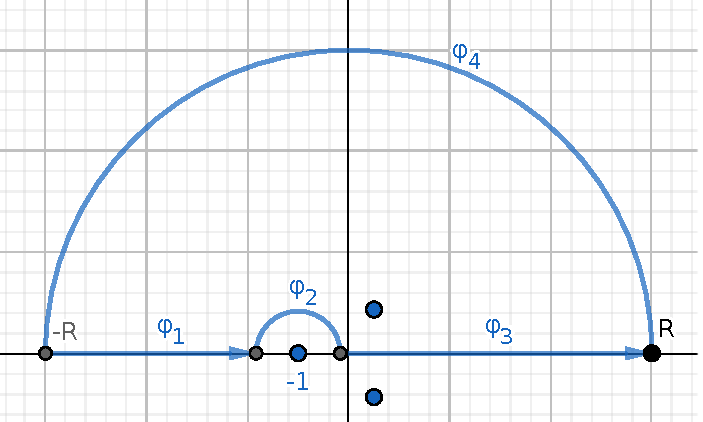
\includegraphics[width=0.6\textwidth]{du2u2param.pdf}
    \label{obr:du2u2param}
\end{figure}
\begin{equation*}
    \varphi = \varphi_1 \oplus \varphi_2 \oplus \varphi_3 \oplus \varphi_4
\end{equation*}
\begin{align*}
    \varphi_1 &= t \mapsto t, t \in [-R, -1 - \nicefrac{1}{R}] \\
    \varphi_2 &= t \mapsto -1 + R^{-1} \e{\i t} \in [\pi, 0] \\
    \varphi_3 &= t \mapsto t, t \in [-1+\nicefrac{1}{R}, R] \\
    \varphi_4 &= t \mapsto R \e{\i t} \in [0, \pi]
\end{align*}
\begin{equation*}
    \int_\varphi f \d{z}
    = \int_{\varphi_1} f \d{z}
    + \int_{\varphi_2} f \d{z}
    + \int_{\varphi_3} f \d{z}
    + \int_{\varphi_4} f \d{z}
\end{equation*}

Nyní použijeme limitní přechod $R\to\infty$ a dostaneme:
\begin{align}
    \int_\varphi f \d{z}
    &= 2\pi\i \Res_{e^{\pi\i/3}} f = \const{konst.}
    \label{residu}
    \\[5pt]
    \int_{\varphi_1} f \d{z} + \int_{\varphi_3} f \d{z}
    &\to \const{p. v.} \int_{-\infty}^{+\infty} f \d{z}
    \\[5pt]
    \int_{\varphi_2} f \d{z} &\to -\pi\i \Res_{-1} f
    \label{kruznic}
    \\[5pt]
    \int_{\varphi_4} f \d{z} &\to 0
    \label{jordan}
\end{align}

Zatímco \eqref{residu} vyplývá z reziduové věty, \eqref{kruznic} vyplývá z tvrzení o obíhání části kružnice a \eqref{jordan} plyne z Jordanovy věty, protože $RM_R \sim R^{-3}$ pro $t>0$ a $\sim R^{-2}$ pro $t = 0$.

Stačí nám tedy vypočíst hodnoty reziduí v bodech $-1$ a $\e{\pi\i/3}$:
\begin{equation*}
    \Res_{-1} f
    = \Res_{-1} \frac{\e{\i tz}}{1 + z^3}
    = \left.\frac{\e{\i tz}}{\dd{}{z} (1 + z^3)}\right|_{z=-1}
    = \frac{\e{-\i t}}{3}
    \\[5pt]
\end{equation*}
\begin{equation*}
    \Res_{\e{\pi\i/3}} f
    = \Res_{\e{\pi\i/3}} \frac{\e{\i tz}}{1 + z^3}
    = \left.\frac{\e{\i tz}}{\dd{}{z} (1 + z^3)}\right|_{z=\e{\pi\i/3}}.
    = \frac{\e{\i t \exp \pi\i/3}}{3\e{2\pi\i/3}}
    = \frac{1}{3} \, \exp \left( \i( \frac{t}{2} - \frac{2}{3}\pi) - \frac{\sqrt{3}}{2}t \right).
\end{equation*}
Dostáváme tedy (pro $t\geq 0$):
\begin{align*}
    I &= \Re\int_\varphi f \d{z} - \Re\int_{\varphi_2} f \d{z}
    = \Re 2\pi\i \exp \left( \i( \frac{t}{2} - \frac{2}{3}\pi) - \frac{\sqrt{3}}{2}t \right) + \Re \pi\i \frac{\e{-\i t}}{3}
    \\
    &= \frac{\pi}{3} \left(
        \sin t - 2 \e{-\frac{\oldsqrt{3}}{2} t} \sin(\frac{t}{2} - \frac{2}{3}\pi)
    \right)
\end{align*}
Nakonec se zbavíme omezení $t\geq 0$ a fuknci sudě rozšíříme:
\begin{equation*}
    \const{p.v.} \int_{-\infty}^{+\infty} \frac{\cos(tx)}{1+x^3} \d{x}
    = \frac{\pi}{3} \left(
        \sin |t| - 2 \e{-\frac{\oldsqrt{3}}{2} |t|} \sin(\frac{|t|}{2} - \frac{2}{3}\pi)
    \right).
\end{equation*}

\end{document}